
\chapter{Introduction}\label{ch:1}
\section{What this study is about}\label{sec:1.1} %1.1 /

Pronunciation in a foreign or second language (L2)\footnote{In the study, I use ``second language'' (L2) as a general term to refer to any kind of ``foreign language''.} is a crucial part of phonological competence and important not only for the learners’ intelligibility but also for assessment of their oral skills. Interest in second language speech is probably as old as second language learning itself and the impact of a learner’s native (first) language on his or her second language has played a central role in it (see, e.g., \citealt{Thomas2013} for a brief history of second language acquisition research). Even though most parts of the grammar may not show major differences in comparison to that of native speakers, second language speech differs from the -- sometimes idealized -- speech of native speakers (\citealt[1]{ColantoniEtAl2015}), with perhaps its most characteristic feature being what is commonly referred to as a “foreign accent”. The main property of this non-native accent is attributed primarily to the features transferred from the first language (L1). While the transfer of L1 segments (consonants and vowels) into L2 production and perception has already received considerable attention (see \citealt{ColantoniEtAl2015, DerwingMunro2015} for overviews), much less is known about how L2 intonation is acquired and how it contributes to the perception of foreign accent by native speakers.


Since intonation serves an important grammatical function, its acquisition is essential. However, it also requires the successful and simultaneous acquisition of other components of language such as segments, syntax, semantics and pragmatics. Aside from its complexity, there is one more way in which the acquisition of intonation differs from the acquisition of other components of language. Whereas non-natives are likely to learn, for instance, the subjunctive in Spanish much later than the indicative (at least in formal instruction), pronunciation (and especially intonation) is present in the acquisition process from the very beginning. The praxis, however, shows that most L2 learners have little or almost no knowledge about how intonation works (this holds true for both their L1 and L2). In general, learners are rarely or never given any training in L2 intonation, which implies that the acquisition of L2 intonation most often occurs intuitively. All these factors may be reasons why intonation is said to be very difficult if not impossible for L2 adult speakers to acquire, whereas it is one of the first aspects of speech that infants attend to, react to and produce themselves (\citealt[74]{Chun1998}, see also \citealt{Grosser1993} and \citealt{Chun2002} for L2 adults’ intonation and \citealt{Snow1998,Snow2006, PrietoEsteve-Gibert2018} for L1 children’s intonation). Yet, on the contrary, intonation is sometimes reported to be a feature of language that we pick up on rapidly when we learn a new language or dialect. Hence, a preliminary question for the present research is: Exactly which features of L2 intonation are learnt first and which later or never? \citet{Bolinger1978} once called intonation “a half-tamed savage” for being difficult to describe and model in comparison to other parts of language (see \sectref{sec:2.2} for a definition of intonation). \citet[50]{Gussenhoven2004} used this metaphor to make a distinction between the \textit{tamed half} linked with the phonological system (intonational grammar) and the \textit{untamed half} that concerns the phonetic implementation of structural elements. It is perhaps not surprising that L2 learners commonly have more problems with the \textit{untamed} \textit{half} of intonation (see \sectref{sec:1.4}).



The present study will examine whether and in which way a foreign intonation can be “tamed” by L2 learners. Its objective is to contribute to a better understanding of the L2 intonation acquisition process by examining F0 contours in L2 Spanish and L2 Italian produced by Czech and German adult learners. The study is descriptive and exploratory in nature as it examines \textit{which features of intonation} are different in the learners’ output; it is at the same time explanatory as it attempts to explain \textit{why} these features are different. The experimental design is closely related to the methods employed by the recent international project (\textit{Inter-})\textit{Fonología del Español Contemporáneo} ((I)FEC, see \citealt{PustkaEtAl2016,PustkaEtAl2018}). All the learners in the present study had received formal instruction in the respective L2s in their home countries, and at the time of the study their proficiency level was between B1–C2 according to the \textit{Common European Framework of Reference for Languages} (CEFR). I did not include any basic-level learners (A1–A2) in the study because their spoken output is limited to basic structures and they are presumably not very fluent in prosody. Moreover, it is known that foreign language beginners concentrate on meaning rather than form \citep{VanPatten1996} -- they are more focused on \textit{what} they say than \textit{how} they say it unless the form has a high communicative value. Additionally, beginners are presumed to be closer to their L1 because their L2 phonological competence is still in the early stages of development and, hence, “it makes much more sense to compare advanced learners with native speakers” \citep[11]{Granger2015}. We can thus assume that when in the course of time learners get more input and start to also focus on form (whether consciously or not), they should improve their phonological skills. The analysis of L2 intonation across proficiency levels (intermediate vs. advanced) can provide an initial glance at how the interlanguage grammar is intonationally constrained at different developmental stages.



In this chapter, I first provide information about the rationale behind the pres\-ent research and highlight its contribution to the field of L2 intonation learning (\sectref{sec:1.2}). Then, after clarifying several core concepts that are necessary for understanding and undertaking L2 speech research in general, I introduce a set of relevant research questions and initial hypotheses (\sectref{sec:1.3}). I continue with an overview of previous and current research in the field, focusing particularly on what constitutes the “foreign” intonational patterns in an L2 (\sectref{sec:1.4}). And finally, I briefly outline the organisation of this manuscript (\sectref{sec:1.5}).


\section{Aims of the present study}\label{sec:1.2}\largerpage %1.2 /

To the best of my knowledge, there are no other studies that examine the impact of one Germanic and one Slavic language on the intonation of two different Romance languages as L2s. The first aim of the present study is to fill a research gap in this respect by offering the first comprehensive contrastive analysis of intonational meaning in Spanish, Italian, German and Czech. It provides a systematic overview of F0 patterns in L2 Spanish and L2 Italian, by focusing on the inventory of pitch accents and boundary tones in different types of sentences set in natural and predetermined contexts.\footnote{Pitch accents refer to the tones associated with the tonic syllable, while boundary tones are the tones associated with the edges of prosodic phrases (see \sectref{sec:2.2}).} Further prosodic parameters such as pitch change (maximal and minimal F0) and duration are considered to some extent too.


Most of the existing studies in this area have focused on only one L1 and one L2 to investigate the acquisition of intonation and test the hypothesis that transfer from one intonation system to another takes place (see \sectref{sec:1.4}). The present study argues that a multidirectional comparison will allow us not only to distinguish L1-dependent features resulting from transfer but also to identify those features common to all learners, regardless of their L1 and the target language \citep[12]{Granger2015}. Hence, the second objective is to apply the \textit{Contrastive Interlanguage Analysis} (CIA) proposed by \citet{Granger1996} in examining two different L1s and two different L2s. The CIA is a two-pronged approach which permits us “to gain a better understanding of the mechanisms of foreign or second language acquisition and to design more efficient language teaching tools and methods” \citep[9]{Granger2015}. Besides its didactic implications, the method can help us to understand the mechanisms of L2 intonation acquisition by uncovering how L1-to-L2 intonational transfer works and what role prosodic similarities and dissimilarities between languages play. There are three scenarios dealt with in the present study (\figref{fig:1:1}, based on \citealt{Granger1996,Granger2015}).




\begin{figure}
%%\includegraphics[width=\textwidth]{figures/a01HabilIntroduction-img001.emf}
\small
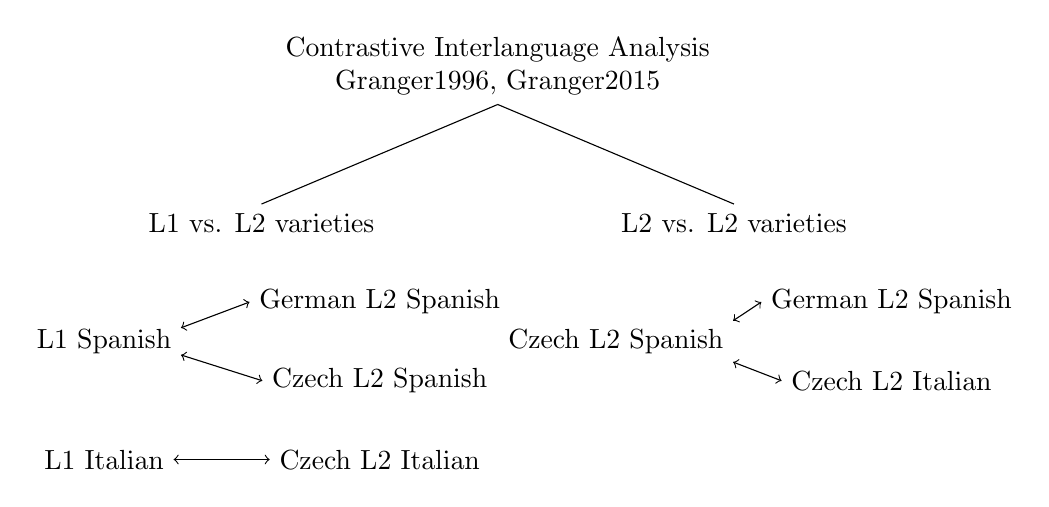
\begin{tikzpicture}[align=center, anchor=center]
\node(top) at (0,5) {Contrastive Interlanguage Analysis\\\citep{Granger1996, Granger2015}};
\node(12) at (-3,3) {L1 vs. L2 varieties};
\node(22) at (3,3) {L2 vs. L2 varieties};
\draw (top.south) -- (12.north);
\draw (top.south) -- (22.north);

\node(1sp) at (-5,1.5) {L1 Spanish};
\node(ge2) at (-1.5,2) {German L2 Spanish};
\node(cz2) at (-1.5,1) {Czech L2 Spanish};
\draw[<->] (1sp.10) -- (ge2.west);
\draw[<->] (1sp.350) -- (cz2.west);

\node(1it) at (-5,0) {L1 Italian};
\node(cz2it) at (-1.5,0) {Czech L2 Italian};
\draw[<->] (1it.east) -- (cz2it.west);

\node(cz2sp) at (1.5,1.5) {Czech L2 Spanish};
\node(ge2r) at (5,2) {German L2 Spanish};
\node(cz2r) at (5,1) {Czech L2 Italian};
\draw[<->] (cz2sp.10) -- (ge2r.west);
\draw[<->] (cz2sp.350) -- (cz2r.west);

\end{tikzpicture}
\caption{Varieties under study according to the \textit{Contrastive Interlanguage Analysis} (based on \citealt{Granger1996,Granger2015}).}
\label{fig:1:1}
\end{figure}

The first scenario involves a comparison of learner data with data from native speakers (L1 Italian vs. L2 Italian, L1 Spanish vs. L2 Spanish). In this instance, I provide basic information about the ways in which the four languages (L1 Spanish, L1 Italian, L1 German, L1 Czech) differ, on the basis of which hypotheses can be formulated. The second scenario includes an analysis of learners from two different language backgrounds (L2 Spanish with L1 Czech vs. L2 Spanish with L1 German). The last scenario examines differences between two different L2s produced by learners of one L1 background (L2 Italian with L1 Czech vs. L2 Spanish with L1 Czech).\footnote{One might note that the scenario “L2 Italian produced by L1 German learners” is lacking here. This is due to the COVID-19 pandemic, which did not allow to carry out the recordings. This L2 variety will be considered in future.} The contrast between all these varieties should clarify not only transferred phenomena but also common tendencies related to the acquisition of L2 intonation in general.


The third aim of the study is to discuss the results within the recently proposed \textit{L2 Intonation Learning theory} (LILt) \citep{Mennen2015}, a theoretical framework designed for intonation. The LILt is based on the Autosegmental-Metrical model of intonational phonology according to which languages differ in four dimensions: tonal inventory, phonetic realization of the tones, function of the tones and the frequency of their occurrence (see \sectref{sec:1.4} and \sectref{sec:2.4}). Here the study hopes to contribute to a better understanding of the interaction of these dimensions by evaluating the intonation patterns of L2 interlanguages in different types of sentence, including (non-)neutral statements, (non-)neutral yes/no questions, \mbox{(non-)}neutral wh-questions and vocatives.



And finally, the present study also contributes to the general discussion related to the modelling and transcribing of intonation, an issue that has been the subject of ongoing debate by applying ToBI (\textit{Tone and Break Indices}), a labelling system for tonal annotation (see \sectref{sec:2.2} and \sectref{sec:3.4.1}), and then discussing the strengths and limitations of this procedure.



The next section introduces various phenomena related to second language speech in general and highlights the key areas that seek to explain L2 behaviour, giving special attention to language transfer and the impact of the L1 on the L2. Based on different core concepts, preliminary questions and expectations related to this study will be formulated.


\section{Second language speech: Terminology and starting hypotheses}\label{sec:1.3}
\subsection{Core concepts}\label{sec:1.3.1}

As explained above, L2 speech refers to non-native production by an individual of a language that was acquired after that person had fully acquired (or nearly so) his/her native or first language(s) (L1).\footnote{The potential influence of another previously acquired L2 -- hence L2 to L3 transfer -- will not be covered in the present study, although the growing field of L3 acquisition has proved that such influences potentially play a role (e.g., \citealt{Odlin1989, CenozEtAl2001, HufeisenFouser2005, DeAngelis2007, Leung2009, WrembelEtAl2010, DeAngelisDewaele2011, GabrielGrünke2018}).} Previous research has looked at the phenomenon of non-native speech from two primary perspectives, one empirical-theoretical (see, e.g., \citealt{Hansen2006} and works cited therein) and the other empirical-didactic (see, e.g., \citealt{LightbownSpada2013}). Whereas the first perspective aims to explain the mechanisms of L2 acquisition as well as individual differences observed in L2 speech, the second one is more concerned with the pedagogical implications and possible strategies for pronunciation instruction in second language teaching. Within the course of the present work, I will focus especially on the main findings from the first area.


In order to understand second language speech and its mechanisms, it is important to first understand some general concepts in second language acquisition (SLA) (see, e.g., \citealt{Brown2000, GassSelinker2008, ColantoniEtAl2015, DerwingMunro2015, VanPattenBenati2015, AlonsoAlonso2018}). \citet[5--16]{TowellHawkins1994} recognize five core areas in explaining L2 behaviour, which will be defined and discussed briefly in turn. It is important to state at the outset that all these inter-related concepts are expected to be relevant for the acquisition of L2 intonation and for formulating the starting hypotheses (\sectref{sec:1.3.2}).



\subsubsection{Incompleteness}
Although in the course of their lives people never lose the ability to learn a new language, it has been widely assumed that after a certain age the majority of L2 learners differ from native speakers of that target language. However, so far there is no consensus in the research on exactly what that age is (see discussion of this topic in \sectref{sec:2.1.3}). \textit{Incompleteness} can be regarded as an L2 end-state grammar, that is, a state beyond which the grammar will not progress further. The end-state grammar characterizes a learner’s ultimate attainment and exhibits different degrees of native-like patterns (\citealt[5]{ColantoniEtAl2015}). Incompletely acquired properties, transfer phenomena or errors in the L2 may result in fossilization or an apparent “cessation of learning” \citep[457]{Odlin2003}, in which some non-native features become stable in a person’s individual way of speaking or writing. Foreign accent may be seen as a product of fossilized L2 pronunciation. The reasons behind the fossilization can be linguistic, neurolinguistic, socio-communicative or instructional in nature (see, e.g., \citealt{Sims1989, HanOdlin2005}). Moreover, \citet{Selinker1993} asserts that fossilization is a type of (predominantly) linguistic simplification that plays -- next to language transfer -- a central role in SLA. In syntax, for example, learners prefer SVO word order over the more complex cleft structures (see, e.g., \citealt{Schachter1988}), and in morphology, learners may simplify the “rich” verbal paradigm of a target language by using fewer or wrong forms independent of their L1 (see, e.g., \citealt{Montrul2011}).



\subsubsection{Cross-linguistic influence (CLI) or language transfer} 
This phenomenon involves all levels of language and is fairly consistently present in all learners. I will use CLI (see \citealt{SharwoodSmithKellerman1986}) and language transfer (see \citealt{Weinreich1953}) interchangeably here to refer to any “influence resulting from the similarities and differences between the target language and any other language that has been previously (and perhaps imperfectly) acquired” \citep[27]{Odlin1989}. Here we should distinguish between positive and negative transfer. \textit{Positive transfer} occurs when L1 and L2 share similarities and learners produce the target language in a native-like manner. \textit{Negative transfer}, on the other hand, occurs when features from the L1 are introduced inappropriately into the L2. Phenomena originating from negative transfer have generally been assumed to be of much greater interest for research purposes, no doubt because transferred dissimilarities are more easily perceived than similarities, though it has been argued (see, e.g., \citealt{Ringbom1987,Ringbom1992}) that positive transfer may affect second language acquisition even more than negative transfer. Differences between the languages at the (phonetic-)phonological level and the resulting (negative) transfer of L1 properties into the L2 contribute significantly to non-native speech.



\subsubsection{Developmental sequences}
This area refers to the fact that L2 learners do not acquire \textit{all} the properties of the L2 at once, since L2 acquisition -- similar to L1 acquisition -- undergoes several stages of development. This means that the learner’s perceptual and productive knowledge changes in the process of acquisition and (mostly) differs from the output we would expect from a native speaker (see, e.g., \citealt{Major1994}). In the theory of SLA this phenomenon is called \textit{interlanguage}, a term coined by \citealt{Selinker1972} (see also \citealt{Selinker1969}). Interlanguage is defined as a separate linguistic system -- an interim grammar between L1 and L2 -- which is “based on the observable output which results from a learner’s attempted production of a TL [target language] norm” \citep[214]{Selinker1972}. In the course of L2 acquisition, the learner develops different interlanguage grammars and strategies, in which further phenomena such as \textit{U-shaped learning patterns} or \textit{overgeneralizations} may emerge. A \textit{U-shaped learning pattern} (see, e.g., \citealt{Abrahamsson2003}) is a non-linear developmental phenomenon observed in individuals not only in L1 and L2 language acquisition but also in very different cognitive areas (see, e.g., \citealt{CarlucciEtAl2005}). As the name implies, learners perform correctly at the beginning of the acquisition process, then their skills descend over time before eventually becoming more accurate again. Errors in this process should not necessarily receive a negative interpretation. \citet{Gershkoff-StoweThelen2004}, who studied infant motor and language development, suggest that the regression in the U-shape development is just “apparent” and merely part of the ordinary mechanisms of change characterized by the collective dynamics of multiple, contingent processes.



One further developmental phenomenon typical of both L1 and L2 language acquisition is \textit{overgeneralization}. This refers to a type of error resulting from the inappropriate application of a rule or pattern and affects all domains of a language (see, e.g., \citealt{R.Ellis1994, WittekTomasello2002, Franceschina2005, GassSelinker2008, MontrulEtAl2010, LightbownSpada2013}). For example, children generally apply regular forms incorrectly to words that require irregular forms or endings (e.g., \textit{speaked} instead of \textit{spoke} in English; \textit{andé} instead of \textit{anduve} ‘I walked’ in Spanish; \textit{ich habe geschlaft} instead of \textit{ich habe geschlafen} ‘I slept’ in German, etc.). We can observe very similar morphological or morpho-syntactic errors in L2 learner productions too. In phonology, learners may overgeneralize segments and probably suprasegments too. For instance, I have observed that some L1 German learners of Spanish tend to pronounce the alveolar trill [r] in contexts where they should use the alveolar tap [ɾ] (e.g., <presente> *[presente] ‘present’). But note that this overgeneralization may actually indicate progress in the learner’s ability to produce the Spanish trill sound [r], which commonly causes difficulty for German native speakers. Overgeneralization can also be understood as a tendency to overshoot or exaggerate the target norm. For example, \citet{Gass1984} reported L1 Italian learners of English exaggerating the VOT English norm, thus pulling away from both native as well as target values (see also \citealt{Flege1980} for a similar tendency in L2 English VOT produced by Saudi Arabians). With respect to intonation, \citet{SantiagoDelais-Roussarie2015a} report L1 German and L1 Spanish learners of French who tend to overshoot final rises at the right edge of non-final clauses in L2 French. Similar overgeneralization of interrogative patterns has also been observed in L1 Italian learners of L2 (Peninsular) Spanish in \citet{GabrielKireva2014a}. As in the case of U-shaped learning, overgeneralization or exaggerating can be viewed positively as an important part of development: “[L]earners first identify \textit{that} there is something to learn and then work out the details, which in many cases involves the maximization of the features of the new element/contrast” \citep[394]{Gass1988}.



\subsubsection{Systematicity}
\begin{sloppypar}
This property is related to the growth in L2 knowledge across learners, which exhibits an interesting parallelism to L1 development. Previous research on different morphological and syntactic phenomena has demonstrated that the same stages or sequences of development can generally be found across different groups of L2 learners, even when they are distinguished by their ages, L1 backgrounds or conditions of exposure to the L2 (see \citealt[11--12]{TowellHawkins1994}). In L2 phonology research, evidence on such “universal” development is reported too. For example, \citegen{Carlisle2001} careful and detailed review of research on syllabic structure acquisition offers evidence that syllable universals have a strong influence on how L2 learners of various L1 backgrounds acquire such structures in different L2s (with the main claims including preference for CV syllables, more frequent modifications of longer margins, less deletion of more sonorous codas, more modifications of margins according to sonority principles, and modification of less preferred margins). Carlisle concludes that there is a “universal” systematic path of (phonological) development independent of L1 and/or the type of input. This does not mean, however, that L1 would not play any important role in the developmental sequences that appear in L2 phonology. As \citet[13]{Ioup1984} and later many others (e.g., \citealt{Shen1990, Wennerstrom1994}) have pointed out, “transfer is \textit{the} major influence on interlanguage phonology”, with a much greater impact here than on interlanguage syntax or other domains. To come back to the example of syllabic structure, Czech-speaking learners of German will have fewer difficulties with acquiring German consonant clusters than, for instance, L1 Spanish or L1 Italian learners. This is because Czech has more complex syllables and codas, whereas Spanish and Italian prefer CV syllables or syllables with simple codas. Hence, transfer processes clearly permit Czech learners to acquire German syllabic structure more rapidly. Also studies on the acquisition of word-stress by French-speaking learners of English (\citealt{Tremblay2008a,Tremblay2008b}, see also \citealt{TremblayOwens2010}) showed that the development of L2 prosodic representations is not random: most of the learners acquired the trochaic foot as they became more proficient in English \citep[168]{Tremblay2008a}. Nonetheless, in general terms more research on different language combinations and cross-linguistic comparisons is still necessary to enable us to explain which phenomena (if any) in prosodic development are universal and which are language-specific. Regarding L2 intonational development, we still lack research here, but see cited works in \sectref{sec:1.4.2}.
\end{sloppypar}


\subsubsection{Variability}\largerpage
This concept implies that L2 learners’ interlanguage systems change over time and go through different stages of variability. L2 learners may variably use two or more forms for a given construction or category. Intermediate speakers in particular can exhibit a very broad inventory of such variation in target sounds or \textit{approximation} attempts (see, e.g., \citealt{Beebe1984}) before they show stabilization in choice of the form. The interlanguage variability occurs either between learners (interlearner variability) or within the same learner (intralearner variability) and its degree is determined by different factors including L1 background, proficiency level, age of L2 learning, role of input and a range of personal reasons. \chapref{ch:2} (\sectref{sec:2.1}) will address all these factors in greater detail.



Similarly as in L1 acquisition, the performance mistakes do not necessarily reflect what L2 learners actually know (i.e., their competence). Indeed, one difficulty for a researcher is not merely to recognize whether a given speaker’s speech contains performance or competence errors (especially in terms of intonation), but also to determine what counts as an error in general (for a discussion on this topic, see, e.g., \citealt{Ringbom1987, GilquinDeCock2011}). When talking about an error in the present study, I will follow a working definition proposed by \citet[57]{DerwingMunro2015}, who define errors as “cases in which a speaker aims to produce an utterance, but as a result of a lack of full control over its segmental or suprasegmental structure, produces something else instead.” This “something else” is mostly a result of cross-linguistic influence. Moreover, while some production errors may be of temporary duration, others may continue over long periods and can lead to fossilization.


\subsection{Starting hypotheses}\label{sec:1.3.2}

Based on the main concepts in SLA presented above and the universal mechanisms of SLA as proposed in \citet{TowellHawkins1994}, the present study makes the following preliminary assumptions.

\begin{description}
\item[Incompleteness hypothesis:] According to this hypothesis, L2 grammar just approaches to the target language and L2 varieties will thus differ from the target languages. Since fossilization makes an important part of the “incomplete” acquisition, several related questions require an answer: What intonational features are candidates for fossilization in L2 speech and why? At what point does fossilization begin?

\item[CLI hypothesis:] It is expected that the learners will exhibit both positive and negative transfer of L1 features and these will be mixed with patterns of the target languages. But will transfer occur in all sentence types and with all tonal elements (pitch accents and boundary tones) in the same way?

\item[Developmental hypothesis:] It was reported that the degree of CLI depends on the stage of L2 development: as L2 development proceeds, L1 transfer effects diminish. The present study expects to find significant differences between intermediate and advanced learners. It is expected that advanced learners will more closely approximate the intonation patterns of the target language. Therefore, L1 Czech and L1 German advanced learners of Spanish should become more similar in their production than intermediate learners. In the same way, advanced learners of L2 Italian will more closely approximate the native-like patterns than intermediate learners. It is also expected that phenomena such as simplification and overgeneralization will arise as evidence of the acquisition strategies and the intonational development.

\item[Systematicity hypothesis:] This hypothesis states that the growth of L2 knowledge will be similar across learners, and similar types of interferences are expected. Another task regarding systematicity and development will be to consider which phenomena might be “universal” and which language-specific.

\item[Variability hypothesis:] The data on L2 intonation predict high (especially interlearner) variation. Though the strength of transfer can have various causes, the present study focuses on L1 background as a main factor and language proficiency as a secondary factor. Other factors such as, for example, the length of experience in a L2-speaking country, are left for the future (see also \sectref{sec:2.1}).
\end{description}

In addition to these basic hypotheses, several \textit{partial hypotheses} related to differences and similarities between L1 and L2 will be developed in the course of the present study. Before highlighting several problematic issues pertaining to the acquisition of L2 intonation and presenting the main findings of some case studies that have focused on L2 Spanish and L2 Italian intonation (\sectref{sec:1.4.2}), I will offer an overview of research concerned with language contact and change (\sectref{sec:1.4.1}). Based on the reported intonation deviations and prosodic transfer in these two areas, several generalizations about L2 behaviour in terms of intonation will be derived.

\section{Previous research on non-native intonation}\label{sec:1.4} %1.4 /
\subsection{L2 intonation in language contact studies}\label{sec:1.4.1}

Interference phenomena play a crucial role in the studies on language contact, which is a major factor in language change, including changes in the domain of phonology (see, e.g., \citealt{Weinreich1953, ThomasonKaufman1988, McMahon2004}). An important point for us here is that most distinctive sound patterns observed in many contact-induced varieties of Spanish and Italian can be seen as products of second-language pronunciation and cross-linguistic influence.


The Spanish language and its long-standing contact with different languages serves as an excellent illustration of diversification based on L1-L2 transfer. One example par excellence is Buenos Aires Spanish, called \textit{Porteño}, which features changes in the prosodic system that were probably triggered by a large Italian immigration in the second half of the 19th century and first third of the 20th (see  \citealt{VidaldeBattini1964, FontanelladeWeinberg1987, Nascimbene1988, Baily1999, Devoto2002}).\footnote{A large majority of Italian immigrants came from either the Piedmont or the South of Italy and spoke mostly regional varieties of Italian and/or Italo-Romance varieties, which were partly mutually unintelligible and led probably to the creation of a linguistic “Babel” (a mixture of these varieties and L2 Spanish).} Several studies devoted to the prosodic aspects of this modern Spanish variety provide empirical evidence that Italian and \textit{Porteño} share several similarities: the early alignment of F0 in prenuclear pitch accents, the final “long fall” in declaratives, the rising-falling boundary tone in yes/no questions and the use of emphatic tritonal pitch accents are the most cited features attributed to the Italian influence (see, e.g., \citealt{Kaisse2001, ColantoniGurlekian2004, GabrielEtAl2010,GabrielEtAl2011, FeldhausenEtAl2011, BenetEtAl2012, PeškováEtAl2012,PeškováEtAl2013}). Interestingly, comparable Italian traces and changes in the prosodic system have also been detected in the Occitan spoken in the Alpine valleys of northwestern Italy \citep{Sichel-BazinEtAl2015}, in the Catalan spoken in the Sardinian city of l’Alguer \citep{PrietoEtAl2015a}, in Tyrolean German \citep{Barker2005} or in the Spanish variety spoken in Mexican Chipilo, where immigrants from northern Italy (Veneto) settled (\citealt{BarnesMichnowicz2015}).



It is assumed that the typological closeness between Italian and Spanish possibly accelerated the creation of a new variety (\citealt[107]{ColantoniGurlekian2004}). Nevertheless, this does not mean that typologically distant languages cannot influence each other. Some examples can be found in Spanish dialects which were in contact with (sub-Saharan) African languages as a consequence of the Atlantic slave trade. By way of illustration, African-influenced intonation patterns have been observed in the vernacular speech of black communities in the Dominican Republic \citep{Megenney1982}. Megenney found that typical declaratives of this community end on a mid tone rather than a falling tone as in other Spanish dialects; this may neutralize the intonational differences between statements and questions. Though a direct influence of African languages on (Dominican) Spanish intonation is not very easy to demonstrate, the different-sounding Spanish dialect points to a possible African substrate impact on the Spanish superstrate. Similar African traces can also be found in the Afro-Iberian creole language \textit{Palenquero} (spoken in the Colombian village of San Basilio de Palenque), which displays a very unique intonation. \citet{HualdeSchwegler2008} show that all prenuclear stressed syllables receive high tones instead of the typical Spanish late peaks in posttonic syllables. A similar “sing-song” intonation and low-high tonal alternations have also been reported in the variety of Spanish spoken in Equatorial Guinea, a former Spanish colony, where Spanish is still a co-official language. The Bantu languages Spanish is in contact with in this area belong to tonal languages characterized by lexical high and low tones (see \citealt{Lipski2005,Lipski2010}). Another contact-induced Spanish dialect with “non-monolingual” intonation patterns is Peruvian Spanish \citep{ORourke2004}, in which (especially Quechua-dominant) bilingual speakers tend to produce prenuclear pitch accents with earlier peaks in the tonic syllable (see also \citealt{Buchholz2021} for Quechua-Spanish contact patterns). Differences in peak alignment have also been observed in Basque-Spanish bilinguals \citep{Elordieta2003} or Spanish-German bilingual children (\citealt{LleóEtAl2004, Lleó2016}).



Besides the above mentioned language contact situations, there are many further studies on intonation, examining, e.g., Yucatecan Spanish in contact with Maya in Mexico \citep{Uth2019}, Spanish-Guaraní contact in Argentina \citep{Colantoni2011} and Paraguay \citep{Pešková2022a}, Spanish-Portuguese contact in Spanish Olivenza \citep{Kireva2016}, Judeo-Spanish in contact with Bulgarian (\citealt{GabrielKireva2014b}), Cuban Spanish in contact with English and other Spanish dialects in Miami \citep{Alvord2006}, Spanish-Catalan contact in Mallorca \citep{Simonet2008} and in Catalonia (\citealt{GrünkeInProgress}). All these studies support the hypothesis that contact-induced changes significantly affect the intonational system (see also \citealt{FrotaPrieto2015} for such influences within other Romance languages; \citealt{Mencken1937} and \citealt{Romaine2001} for a brief remark on the intonation of Pennsylvania German English; \citealt{Grenoble2010} for intonational influences in Slavic languages; \citealt{Birkner2004} for influence of Portuguese in Brazilian German bilinguals; and many other examples).



With regard to contact-induced changes in (the regional varieties of) Italian, \citet{Cerruti2011},  \citet{GiliFivelaEtAl2015} -- among many others -- suggest prosodic influences from the contact with local vernaculars all over Italy. For example, the regional varieties of Italian spoken in Sardinia share intonational similarities (e.g., falling patterns in yes/no questions) with Sardinian \citep{VanrellEtAl2015}. In the same fashion,  \citet{RoseanoFernándezPlanas2019} report similarities between Friulian, and the regional Italian variety spoken in the town Tolmezzo in the autonomous Friuli-Venezia Giulia part of Italy (see also  \citealt{FernándezPlanasEtAl2017}). It should be added that although the Italian phonological system is known for being very heterogeneous,  \citet[196]{GiliFivelaEtAl2015} claim that stereotypical patterns, meaning “patterns shared by many (maybe all) varieties” do exist (e.g., the fall from a high pretonic syllable to a low tone in neutral statements or the early peak alignment used for contrastive-correction focus; see \chapref{ch:4}).



What do we learn from all these contact situations for the present study? First, they support the starting hypotheses formulated in \sectref{sec:1.3}. As we saw, intonation patterns undergo modifications through language contact, and CLI may accelerate such changes, which can significantly affect the prosodic system. Second, the heterogeneity resulting from language changes and development is patterned. Third, languages in contact do not show a one-to-one transfer, but rather the creation of mixed systems, “innovative hybrids” \citep{Lipski2010} or “fusion-like” patterns \citep{Queen2001} which derive from the contact environment. Hence, the interlanguages differ clearly from both the native language and the target language (see, e.g., \citealt{Tarone1987}) and not all deviations are necessarily due to interferences (see, e.g., \citealt{KielhöferJonekeit2018}).



Since intonational variation and change observed in contact language situations are connected with interlanguages, I expect similar behaviour and principles that govern changes in intonation and the mechanisms of the acquisition processes in my data too. This raises questions about the extent to which intonation is learnable, what patterns from the L1 are transferred into the L2, and, importantly, whether there are limitations on the transfer, and if so, where they are and why they exist.


\subsection{L2 intonation in SLA studies}\label{sec:1.4.2}

As yet, research in SLA on phonology and especially intonation is considerably limited when compared with other domains of language. Our growing knowledge in the field of L1 intonation especially during the last two decades has resulted in an increased interest in L2 intonation acquisition too. However, an overwhelming number of studies on non-native intonation concern L2 English produced by speakers with various language backgrounds (see, e.g., \citealt{Barlow1998, Gut2009, Mennen2007,Mennen2015, MennendeLeeuw2014, Puga2019,Puga2021} for overviews). Only a smaller number of studies are devoted to non-native intonation in L2 Spanish and L2 Italian, and -- to the best of my knowledge -- none of these studies have taken into account learners with L1 Czech. The aim of this section is to present a summary of the main current research findings with a focus on Spanish and Italian.

\begin{sloppypar}
Already  \citet[7]{NavarroTomás1948} remarked that intonation represents the “greatest stronghold” in the acquisition of a foreign language. One of the first em\-pir\-i\-cal\-ly-ori\-ent\-ed investigations of non-native Spanish intonation were carried out by \citet{Cantero1994} and \citet{CortésMoreno1998, CortésMoreno2001}, who offer preliminary descriptions of different (Peninsular) Spanish tonal contours and place the focus on didactical issues, which should allow the learners to gain not only linguistic but also communicative and intercultural competences. The nature of possible difficulties in learning intonation and its development are also taken into account. For example, Cortés Moreno reports interesting results for L2 Spanish produced by L1 Chinese learners, revealing that they acquire Spanish intonation in the following order: declarative sentences > wh-questions > yes/no questions > exclamatory (emphatic) sentences. This observation implies that the acquisition of intonation is constrained and indicates in which area intonational difficulties and deviations may occur. The broad explanation pursued by Cortés Moreno is that the acquisition hierarchy is due to both positive and negative transfer from L1.
\end{sloppypar}



More recently, \citet{AstrucVanrell2016} have contributed to the field with their study on the acquisition of politeness and intonation, which examines semi-spontaneous data produced by L1 English (beginning-level) learners of L2 Spanish. Based on acoustic analysis couched within the AM approach, they found out that the learners applied sociopragmatic knowledge and formulated pragmatically appropriate speech acts relatively well, but differed from Spanish natives in the distribution and frequency of tonal accents and their phonetic realisation. Other studies provide evidence that L1 transfer is an important factor in the production of L2 intonation (see, e.g., \citealt{Radel2008} for cross-linguistic influence in L2 Spanish declaratives and yes/no questions produced by L1 German learners; \citealt{GabrielKireva2014a} for “Italian” boundary tones in L2 Spanish yes/no questions; \citealt{JunEtAl2018} for difficulties in the phonetic implementation of the prenuclear rising F0 contours in L2 Spanish statements produced by L1 Korean learners; \citealt{vanMaastricht2018} for the acquisition of focus marking in L2 Spanish produced by L1 Dutch learners).



Another group of studies within the AM framework provide a window onto the development of L2 intonation by examining tonal patterns of L1 English native learners of different Spanish dialects in a study abroad context (e.g., \citealt{HenriksenEtAl2010} for the Spanish of León in Spain; \citealt{Trimble2013} for the Spanish of Mérida in Venezuela; \citealt{Craft2015} for Valencian Spanish; \citealt{Buck2016} for Salamanca Spanish in Spain; and  \citealt{MéndezSeijas2018} for the variety of Spanish spoken in Barcelona). These studies prove that learners increasingly approximate target-like intonation in the course of time, although not all exhibit significant changes. This general finding is important because it means that intonation is learnable and that learners approximate the variety they are exposed to. A further conclusion is that CLI remains present to different degrees and that learners do not attain native productions completely: avoidance of \textit{uptalk} (a high-rising terminal) in statements, later peak alignment of prenuclear pitch accents and different types of boundary tones represent a particular difficulty at least for L1 English learners. However, intonation development does not affect all phenomena in the same way and exhibits individual differences. For example,  \citet{MéndezSeijas2018} observed that whereas some learners improved their production of boundary tones after a five-week immersion experience (see also \citealt{Zárate-Sández2018}), they did not exhibit notable changes in prenuclear positions. Méndez Seijas offers an explanation for this within the \textit{L2 Intonation Learning theory} (see more below): fossilization in the peak alignment of prenuclear pitch accents occurs due to the perceptual similarities between Spanish and English and the fact that the contours in this position do not change meaning. In contrast, the drop of English \textit{uptalks} over time can be linked with the “strong semantic weight” involved. In other words, the learners are forced to acquire the target pattern of statements in Spanish (here the falling contour) properly because rising patterns can be confused with a question.



With regard to the research on L2 Italian intonation (see  \citealt{DevísHerraiz2008, DeMeoPettorino2012} and \citealt{Nicora2020} for overviews), we can organise the work done roughly into two main groups: studies that adopt the AM framework (e.g., \citealt{AvesaniEtAl2015, TurcoEtAl2015, NicoraEtAl2019}) and practice-oriented studies (e.g., \citealt{PettorinoEtAl2012, DeMarcoEtAl2014, Mocciaro2014, ViglianoEtAl2016}). Independently from the approach, most of the studies aim to highlight difficulties related to intonation learning, by providing contrastive analysis of Italian and different languages. They also provide evidence of developmental sequences that move towards native-like patterns according to the differences observed between proficiency levels that learners mostly achieved through formal instruction. Similarly to research on L2 Spanish intonation, studies on L2 Italian intonation demonstrate the relevance of L1 to non-native speech and support the prosodic transfer hypothesis (e.g.,  \citealt{DevísHerraiz2008,DevísHerraiz2011} for the acquisition of declaratives and interrogatives in L2 Italian produced by L1 Spanish speakers; \citealt{CroccoBaele2012} for the development of the phonetic implementation of the rises in yes/no questions by L1 (Belgian) Dutch learners; \citealt{Mocciaro2014} for the acquisition of Italian wh-questions and yes/no questions by L1 Vietnamese learners; \citealt{AvesaniEtAl2015} for the acquisition of givenness and focus marking in L2 Italian produced by L1 German learners and vice versa; \citealt{TurcoEtAl2015} for the polarity contrast in L2 Italian produced by L1 German and L1 Dutch learners; \citealt{VitaleEtAl2017} for yes/no questions in L2 Italian produced by L1 Chinese learners; and \citealt{NicoraEtAl2018} for Italian yes/no questions produced by L1 (Irish) English speakers). Furthermore, the works on L2 Italian place a special emphasis on teaching and learning Italian as a foreign language and offer several production/perception-based or imitation-based techniques that should help learners to obtain native-like intonation patterns. For example, the recent studies by \citet{NicoraEtAl2018, NicoraEtAl2019} demonstrate positive effects of a specific training in L1 Hiberno-English learners of Italian. The training consisted in raising prosodic awareness and contrastive L1-L2 analysis, imitation tasks, self-recordings and auto-corrections with the visual support of Praat software. The authors nicely show an improvement in two tested areas, lexical stress placement and intonational patterns of broad focus declaratives and information-seeking yes/no questions.



The present study attempts to generalize the main findings from the above-mentioned research on L2 Spanish and L2 Italian (see also \citealt{Mennen2007,Mennen2015} for further language combinations), which all report intonation cross-linguistic influence. The following key points will all be developed further in the course of the study:


\begin{itemize}
\sloppy
\item Intonational transfer is attested with both pitch accents and boundary tones in different types of sentence.

\item Phonological features of intonation are acquired earlier than the phonetic control of pitch.

\item Difficulties in the phonetic domain concern especially pitch alignment, pitch range and pitch timing.

\item Pragmatically marked structures are acquired later than neutral structures.

\item Patterns with a strong semantic weight are acquired earlier than patterns with no changes in meaning.

\item Patterns that exist in both L1 and L2 are acquired earlier than new patterns.

\item L2 intonation can be improved by appropriate learning\slash teaching techniques.

\item L2 intonation is full of interlearner variation and prosodic development is mostly individual.

\item L1 based-transferred and/or mixed interlanguage patterns undergo stabilization over time.
\end{itemize}

In order to test such L2 behaviour and to understand the learning mechanisms of L2 intonation, the present study will interpret the results within the recent -- and to the best of my knowledge -- so far only model designed for the acquisition of intonation in a second language: The \textit{L2 Intonation Learning theory} \citep{Mennen2015}. The LILt can be understood as a “working model […] that aims to account for the difficulties that L2 learners encounter in producing L2 intonation” \citep[171]{Mennen2015}. This model recognizes four dimensions, in which languages (may) differ and from which predictions on intonation deviations can be made: (1) the systemic dimension, which concerns the inventory and distribution of structural phonological elements, (2) the realisational dimension, which refers to the phonetic implementation of such elements, (3) the semantic dimension, which refers to the function or meaning of the elements; and (4) the frequency dimension, which refers to the frequency of use of the elements. Moreover, the LILt suggests that these intonation dimensions do not create the same amount of difficulty in L2 learning. The main goal is to explain the nature of these difficulties and to discover whether and how contrasts between L1 and L2 play a role in them. Expanding on L2 perception-based models for segmental speech learning (\sectref{sec:2.4}), the LILt also postulates that most intonation deviations and difficulties may be perceptually motivated and that the degree of perceptual similarity is determined by the semantic dimension. It also underlines that tonal contrasts must be controlled for in terms of position and context (all these aspects and further details on the LILt will be presented in \sectref{sec:2.4}). Basing on the previous research as well as the findings of the present study couched within the LILt, I will propose a \textit{Developmental L2 Intonation Hypothesis} (\sectref{sec:5.4}) which seeks to capture the “universal” characteristics of interlanguage intonation development independently of learners’ L1 backgrounds and L2. It is my hope to contribute with this study to the understanding of this still relatively underrepresented area of second language acquisition.

\section{Organisation of the study}\label{sec:1.5}  %1.5 /

The study is organised in six chapters. \chapref{ch:2} consists of four main sections which lay the theoretical foundation for the topic of the present research. First, the findings from both theoretical and empirical research on important factors shaping L2 speech are presented and discussed (\sectref{sec:2.1}). The following section (\sectref{sec:2.2}) offers a definition on intonation and talks about how the prosodic structure of spoken utterances can be modelled. Special focus is placed on the ToBI labelling system, grounded in the Autosegmental Metrical model of intonational phonology, which will be applied in the present study. In \sectref{sec:2.3}, I will compare the phonological systems of the languages under study, including their segmental and suprasegmental properties. The last section of the chapter turns to the models and theories that researchers have developed for the analysis of L2 speech. \citegen{Lado1957} \textit{Contrastive Analysis Hypothesis} and \citegen{Mennen2015} \textit{L2 Intonation Learning theory} are at the centre of attention here (\sectref{sec:2.4}). In order to answer the research questions that guide the present study, L1 and L2 data were collected by means of a production experiment with a total of sixty learners and twelve (Spanish and Italian) controls. A description of the experiment, its design (\sectref{sec:3.1}), participants (\sectref{sec:3.2}), experimental procedure (\sectref{sec:3.3}), intonational analysis and acoustic measurements (\sectref{sec:3.4}) are given in \chapref{ch:3}.

\chapref{ch:4} is the core of the study. It describes the main results on F0 contours in L2 Spanish and L2 Italian, produced by L1 Czech and L1 German learners. The chapter has five sections in accordance with the sentence types analysed: neutral statements (\sectref{sec:4.1}), non-neutral statements (\sectref{sec:4.2}), yes/no questions (\sectref{sec:4.3}), wh-questions (\sectref{sec:4.4}) and vocatives (\sectref{sec:4.5}). Every section begins with a contrastive analysis between L1 and L2, from which a series of CLI hypotheses are derived, then presents L2 outcomes providing illustrative examples of intonational contours and concludes with a summary and discussion.

\chapref{ch:5} offers an overall summary and general discussion of the most salient findings, which include the differences between L2 learner varieties (\sectref{sec:5.1}), the accuracy of L2 intonation patterns (\sectref{sec:5.2}), the deviations in four dimensions of intonation assumed in the LILt (\sectref{sec:5.3}) and issues related to the developmental sequences (\sectref{sec:5.4}). Concluding remarks, recommendations and future directions for research are stated in \chapref{ch:6}.
